\documentclass[conference]{IEEEtran}
\usepackage{cite}
\usepackage{amsmath,amssymb}
\usepackage{graphicx}
\usepackage{booktabs}
\usepackage{xcolor}
\usepackage{tikz}
\usetikzlibrary{positioning,arrows.meta,fit,backgrounds}
\usepackage{placeins}
\usepackage[hidelinks]{hyperref}
\graphicspath{{figures/}}

\begin{document}

\title{FAENet: A Fairness-Aware Evidential Neural Network with Uncertainty-Based Human Review for Employee Attrition Prediction}

\author{\IEEEauthorblockN{Lakshya Varshney}
\IEEEauthorblockA{Department of Computer Science and Engineering\\
Student ID: 2310110513}
\and
\IEEEauthorblockN{Akash Agarwal}
\IEEEauthorblockA{Department of Computer Science and Engineering\\
Student ID: 2310110718}}

\maketitle

\begin{abstract}
Employee attrition raises recruitment and training costs and disrupts teams, so organisations increasingly use machine learning to identify employees who may leave. A useful attrition model must do more than rank employees: it should express how much evidence supports each prediction, detect actual leavers at similar rates across employee groups, and send doubtful cases to a human reviewer. This paper presents FAENet, a fairness-aware evidential neural network built for these three goals. FAENet is an ensemble of five evidential networks that output Dirichlet evidence for the two classes, giving an attrition probability and an uncertainty score for every employee. Training combines a class-weighted evidential loss, an annealed evidence regulariser and a differentiable equal-opportunity penalty on group true-positive rates. At decision time, the most uncertain cases are referred to human review under group-balanced thresholds, and optional age-aware decision thresholds equalise leaver detection across age groups. On the IBM HR Analytics dataset, evaluated with five-times repeated five-fold cross-validation and employee-level bootstrap confidence intervals, FAENet is compared with a single evidential network baseline. FAENet raises ROC-AUC from 0.814 to 0.827, PR-AUC from 0.575 to 0.604 and precision from 0.520 to 0.549. With age-aware thresholds, detection of leavers aged 40 and above rises from 0.365 to 0.565 and the age-band detection gap falls from 0.297 to 0.077. The evidential uncertainty identifies misclassified employees with an AUROC of 0.790 against 0.612 for the baseline, and reviewing the 10\% most uncertain cases lowers the remaining error from 0.149 to 0.105.
\end{abstract}

\begin{IEEEkeywords}
employee attrition, evidential deep learning, algorithmic fairness, uncertainty estimation, human-in-the-loop, deep ensembles
\end{IEEEkeywords}

\section{Introduction}
\subsection{Motivation}
Unplanned employee departures affect continuity, recruitment expenses, training costs and organisational knowledge. Human resources (HR) analytics therefore uses historical employee records to estimate who is likely to leave, so that retention measures can start early. Machine learning (ML) models for this task are now common \cite{talebi2025,alakasheh2024decade}, and recent studies add explanations, threshold calibration and fairness audits \cite{jia2026,alali2026,chaudhary2025}.

\subsection{Problem}
Most attrition models return a single risk score. That score does not tell an HR professional how much evidence supports it, whether the model detects leavers equally well in every employee group, or which predictions should be checked by a person before any action. A model that is accurate on average can still miss many leavers in a minority group, and a confident-looking score can rest on very little evidence.

\subsection{Objectives}
This project set five objectives:
\begin{enumerate}
\item build a neural attrition model that outputs a probability and an uncertainty score for every employee;
\item handle the minority attrition class while keeping probabilities well calibrated;
\item reduce differences in true-positive rate (TPR) across age and gender groups;
\item refer uncertain predictions to human review in a way that is balanced across groups;
\item explain predictions and validate every result with repeated, paired statistical testing.
\end{enumerate}

\subsection{Contributions}
\begin{itemize}
\item \textbf{FAENet}, a cross-fitted ensemble of evidential neural networks (EDL) \cite{sensoy2018} with engineered tenure and satisfaction features, giving a probability, an evidential uncertainty and an ensemble-disagreement score.
\item A \textbf{fairness-aware training objective} with a differentiable equal-opportunity penalty \cite{hardt2016}, compared against Group Distributionally Robust Optimisation (Group DRO) \cite{sagawa2020} and fairness-aware checkpoint selection.
\item \textbf{Age-aware decision thresholds} that equalise leaver detection across age bands, and a \textbf{group-balanced human-review rule} driven by evidential uncertainty, with a learned review head for comparison.
\item A \textbf{rigorous evaluation} on the IBM HR Analytics dataset with 5$\times$5 repeated cross-validation, paired employee-level bootstrap confidence intervals (CIs), unseen-group tests and SHapley Additive exPlanations (SHAP).
\end{itemize}

\section{Related Work}
\subsection{Prior Studies}
\textbf{Attrition prediction.} Systematic reviews cover logistic regression, decision trees, random forests, support vector machines, neural networks and ensembles, and repeatedly identify overtime and job satisfaction as key predictors \cite{talebi2025,alakasheh2024decade}. Jia \cite{jia2026} combines SHAP explanations, threshold calibration and a demographic fairness audit, and reports an XGBoost ROC-AUC of 0.773 on IBM. Al-Ali et al.\ \cite{alali2026} integrate class-imbalance handling, feature selection and SHAP. Chaudhary et al.\ \cite{chaudhary2025} evaluate transparency in churn prediction with explainable AI. Neural networks \cite{wu2024}, knowledge graphs \cite{alakasheh2024kg} and organisation-specific models \cite{varkiani2025} have also been studied.

\textbf{Uncertainty, review and fairness.} EDL \cite{sensoy2018} places a Dirichlet distribution over class probabilities, giving uncertainty from a single forward pass; deep ensembles \cite{lakshminarayanan2017} estimate uncertainty from member disagreement. Selective classification \cite{geifman2017} and learning to defer \cite{madras2018} decide when a model should hand a case to a person. Equal opportunity \cite{hardt2016} requires equal TPR across groups, Group DRO \cite{sagawa2020} minimises the worst group's loss, and selective prediction can magnify group disparities if it is not audited \cite{jones2021}. Recent work combines evidential models and fairness in other domains \cite{barker2026,chen2026faml,chen2025ufare}. Neural network probabilities also need calibration \cite{guo2017,platt1999}.

\subsection{Research Gap}
Existing attrition studies address accuracy and explanation, and some audit fairness after training. None combines, in one neural model, evidential uncertainty, fairness enforced during training, group-balanced human review and age-aware decisions, evaluated with repeated paired testing. Table~\ref{tab:prior} summarises this gap; FAENet is the only approach that covers every capability.

\begin{table}[t]\centering
\caption{Capabilities of FAENet compared with prior attrition studies}\label{tab:prior}
\scriptsize\setlength{\tabcolsep}{2.5pt}
\resizebox{\columnwidth}{!}{\begin{tabular}{lcccccc}\toprule
Study & Model & SHAP & Uncert. & Fair train. & Review & Repeated CV\\\midrule
Jia \cite{jia2026} & XGBoost & \checkmark & & audit only & & \\
Al-Ali et al.\ \cite{alali2026} & Boosting & \checkmark & & & & \\
Chaudhary et al.\ \cite{chaudhary2025} & LR / RF & \checkmark & & & & \\
Al Akasheh et al.\ \cite{alakasheh2024kg} & KG + GCN & \checkmark & & & & \\
Wu and Fukui \cite{wu2024} & NN and others & \checkmark & & & & \\
\textbf{FAENet (ours)} & Evidential NN ens. & \checkmark & \checkmark & \checkmark & \checkmark & \checkmark\\
\bottomrule\end{tabular}}
\end{table}

\section{Methodology}
\subsection{Approach}
FAENet treats attrition prediction as evidence estimation rather than plain classification. Each employee record is mapped by an ensemble of evidential neural networks to Dirichlet evidence for the two classes, which yields an attrition probability, an uncertainty score and an ensemble-disagreement score. Fairness is built into training through an equal-opportunity penalty and into decisions through age-aware thresholds, and the uncertainty score drives a group-balanced human-review rule. SHAP explains both the risk and the uncertainty of each prediction. The following subsections describe the architecture, the training and decision algorithms, and the dataset.

\subsection{Architecture}
Fig.~\ref{fig:arch} shows the FAENet pipeline. Each ensemble member is a multilayer perceptron (MLP) with layers $d\rightarrow32\rightarrow16\rightarrow2$, rectified linear unit (ReLU) activations and dropout 0.1. For input $x$ the member outputs logits $z\in\mathbb{R}^2$, converted into non-negative evidence and Dirichlet parameters:
\begin{equation}
e_k=\mathrm{softplus}(z_k),\qquad \alpha_k=e_k+1,\qquad k\in\{0,1\},
\end{equation}
where class 1 denotes attrition. With total concentration $S=\alpha_0+\alpha_1$, the attrition probability and evidential uncertainty are
\begin{equation}
p=\frac{\alpha_1}{S},\qquad u=\frac{K}{S}=\frac{2}{S},
\end{equation}
where $K=2$ is the number of classes; $u$ is high when little evidence has been accumulated.

\begin{figure}[t]\centering
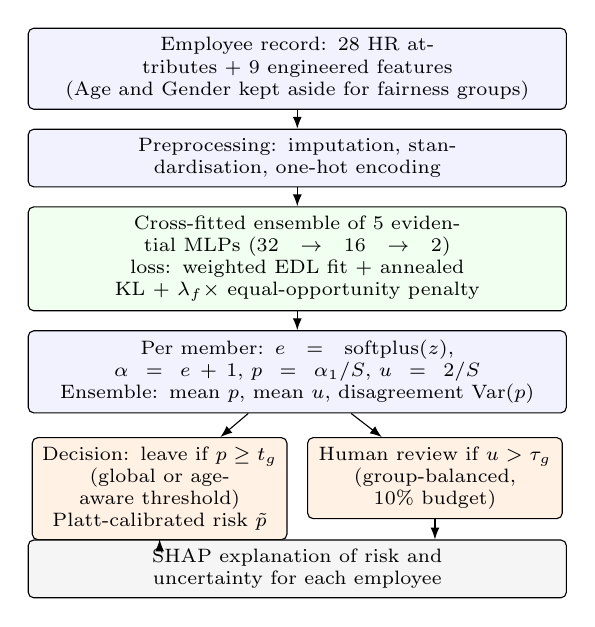
\begin{tikzpicture}[node distance=2.4mm, every node/.style={font=\scriptsize}, b/.style={draw, rounded corners=2pt, align=center, minimum height=5.5mm, fill=blue!5, text width=6.6cm}, s/.style={draw, rounded corners=2pt, align=center, minimum height=5.5mm, fill=orange!10, text width=3.0cm}, a/.style={-{Latex[length=1.5mm]}}]
\node[b] (in) {Employee record: 28 HR attributes + 9 engineered features\\(Age and Gender kept aside for fairness groups)};
\node[b, below=of in] (pre) {Preprocessing: imputation, standardisation, one-hot encoding};
\node[b, below=of pre, fill=green!6] (ens) {Cross-fitted ensemble of 5 evidential MLPs ($32\rightarrow16\rightarrow2$)\\loss: weighted EDL fit + annealed KL + $\lambda_f\times$ equal-opportunity penalty};
\node[b, below=of ens] (dir) {Per member: $e=\mathrm{softplus}(z)$, $\alpha=e+1$, $p=\alpha_1/S$, $u=2/S$\\Ensemble: mean $p$, mean $u$, disagreement $\mathrm{Var}(p)$};
\node[s, below left=3mm and -33mm of dir] (dec) {Decision: leave if $p\geq t_g$\\(global or age-aware threshold)\\Platt-calibrated risk $\tilde p$};
\node[s, below right=3mm and -33mm of dir] (rev) {Human review if $u>\tau_g$\\(group-balanced, 10\% budget)};
\node[b, below=16mm of dir, fill=gray!8] (exp) {SHAP explanation of risk and uncertainty for each employee};
\draw[a] (in)--(pre); \draw[a] (pre)--(ens); \draw[a] (ens)--(dir); \draw[a] (dir)--(dec); \draw[a] (dir)--(rev);
\draw[a] (dec)--(exp.north -| dec); \draw[a] (rev)--(exp.north -| rev);
\end{tikzpicture}
\caption{FAENet architecture and decision pipeline.}\label{fig:arch}
\end{figure}

\subsection{Algorithms}
\subsubsection{Training Objective}
Each member minimises
\begin{equation}
L=\frac{1}{B}\sum_{i=1}^{B}w_{y_i}L_{\mathrm{fit},i}+\lambda_r(t)\,\overline{L}_{\mathrm{KL}}+\lambda_f L_{\mathrm{fair}},
\end{equation}
where $B$ is the batch size. The evidential fit term \cite{sensoy2018} is
\begin{equation}
L_{\mathrm{fit},i}=\sum_{k}\Big[(y_{ik}-p_{ik})^2+\frac{p_{ik}(1-p_{ik})}{S_i+1}\Big],
\end{equation}
with one-hot labels $y_{ik}$. Class weights $w_c=(N/2N_c)^{\gamma}$ with $\gamma=0.5$ give the minority class more influence while keeping probabilities close to observed rates; $N$ is the number of training employees and $N_c$ the number in class $c$. The regulariser $L_{\mathrm{KL}}=\mathrm{KL}[\mathrm{Dir}(\tilde\alpha)\,\|\,\mathrm{Dir}(\mathbf{1})]$ with $\tilde\alpha=y+(1-y)\odot\alpha$ removes misleading evidence, and its weight is annealed as $\lambda_r(t)=\min(1,t/10)\,\lambda_r$.

\textbf{Equal-opportunity penalty.} For group $g$ of attribute $a$ (age band or gender), the soft TPR is the mean predicted probability over the group's actual leavers,
\begin{equation}
\widehat{TPR}_g=\frac{\sum_i \mathbb{1}[A_i=g]\,y_i\,p_i}{\sum_i \mathbb{1}[A_i=g]\,y_i},
\end{equation}
and the penalty sums squared differences from the reference groups $r_a$ (30 to 39 years; male):
\begin{equation}
L_{\mathrm{fair}}=\sum_{a}\sum_{g\neq r_a}\big(\widehat{TPR}_g-\widehat{TPR}_{r_a}\big)^2.
\end{equation}
It is computed over all training leavers at every step, which gives stable group estimates. Group DRO \cite{sagawa2020}, which reweights the 12 gender $\times$ age $\times$ class cells towards the worst-performing one, and fairness-aware checkpoint selection were evaluated as alternatives.

\subsubsection{Ensemble, Decisions and Review}
The training data of each split is divided into five inner folds; member $k$ is trained without fold $k$ and early-stopped on validation PR-AUC. This cross-fitting gives every training employee an out-of-fold prediction, used to train a learned review head. The classification threshold $t_y$ maximises validation F1. \textbf{Age-aware thresholds} $t_g$ are set per age band on validation data so that each band reaches the overall validation TPR. Platt scaling \cite{platt1999} of the logit of $p$, fitted on validation data, gives calibrated risks $\tilde p$. For review, a case is referred when its score exceeds $\tau_g$, the validation quantile that refers 10\% of employees within age band $g$. Five review scores are compared: evidential $u$, entropy of $p$, ensemble disagreement, margin to the threshold $1-|p-t_y|/\max(t_y,1-t_y)$, and the learned review head, a small MLP that predicts misclassification from $[x,\mathrm{logit}\,p,u]$ \cite{madras2018}.

\subsection{Dataset}
We use the IBM HR Analytics Employee Attrition and Performance dataset \cite{ibmdata}: 1{,}470 employees described by 35 attributes, of whom 237 (16.1\%) left. The identifier and three constant columns are removed. \texttt{Age} and \texttt{Gender} are kept out of the model inputs and are used only to define fairness groups; age is grouped into $<$30, 30 to 39, and 40+ years. Nine engineered features are added: log income, tenure ratio (years at company over total working years), years in current role and with current manager relative to tenure, promotion recency relative to tenure, income per job level, companies per working year, the sum of the five satisfaction ratings, and years worked before joining. Numeric features are median-imputed and standardised, and categorical features are one-hot encoded, with all statistics fitted on training data.



\section{Results and Discussion}
\subsection{Experimental Setup}
All models are evaluated with five repeats of stratified five-fold cross-validation (25 splits), stratified jointly on attrition, gender and age band. In each split one fold is the test set and 15\% of all employees form the validation set used for early stopping, thresholds, calibration and review quantiles. The five test folds of a repeat score every employee once; metrics are computed per repeat and averaged, and 95\% CIs come from 500 bootstrap resamples of employees. Model comparisons are paired on identical employees and splits. Hyperparameters were selected on validation folds (Table~\ref{tab:hp}). Implementation uses Python and PyTorch.

\begin{table}[t]\centering
\caption{Selected FAENet hyperparameters}\label{tab:hp}
\scriptsize\begin{tabular}{ll}\toprule
Parameter & Value\\\midrule
Hidden layers & 32, 16 (ReLU, dropout 0.1)\\
Ensemble & 5 cross-fitted members\\
Optimiser & AdamW, lr $10^{-3}$, weight decay $10^{-3}$\\
Batch size, max epochs, patience & 64, 200, 15\\
Class-weight exponent $\gamma$ & 0.5\\
KL weight $\lambda_r$, annealing & 0.5, 10 epochs\\
Fairness weight $\lambda_f$ & 30\\
Review budget & 10\% per age band\\
\bottomrule\end{tabular}
\end{table}

\subsection{Evaluation Metrics}
We report ROC-AUC, PR-AUC (suited to the 16\% attrition rate), precision, recall, F1-score, expected calibration error (ECE) and the Brier score \cite{brier1950} after Platt scaling. Fairness is measured by the TPR gap, the difference between the highest and lowest TPR over the three age bands, and by the TPR of leavers aged 40+. Uncertainty is measured by the AUROC with which $u$ separates misclassified from correctly classified employees, and review quality by the error that remains after the 10\% most uncertain employees are referred.

\subsection{Baseline}
The baseline is a single evidential network with the original feature set and full inverse-frequency class weights, evaluated on exactly the same 25 splits. Table~\ref{tab:main} reports both models with paired 95\% CIs.

\begin{table}[t]\centering
\caption{Baseline (single evidential network) versus final FAENet. Mean over 5 repeats of pooled out-of-fold predictions; $\Delta$ with 95\% paired employee-level bootstrap CI. Fairness rows use FAENet's age-aware thresholds; the review row refers the 10\% most uncertain employees.}\label{tab:main}
\scriptsize\setlength{\tabcolsep}{3pt}\resizebox{\columnwidth}{!}{\begin{tabular}{lccc}\toprule
Metric & Baseline & \textbf{FAENet} & $\Delta$ [95\% CI]\\\midrule
\multicolumn{4}{l}{\textit{Prediction}}\\
ROC-AUC & 0.814 & \textbf{0.827} & +0.013 [+0.004, +0.024]\\
PR-AUC & 0.575 & \textbf{0.604} & +0.029 [+0.006, +0.055]\\
F1-score & 0.538 & \textbf{0.548} & +0.009 [-0.010, +0.033]\\
Precision & 0.520 & \textbf{0.549} & +0.029 [+0.007, +0.052]\\
Recall & 0.559 & \textbf{0.547} & -0.012 [-0.035, +0.015]\\
\midrule\multicolumn{4}{l}{\textit{Calibration}}\\
ECE (calibrated) & 0.030 & \textbf{0.020} & -0.010 [-0.014, +0.001]\\
Brier score (calibrated) & 0.101 & \textbf{0.095} & -0.006 [-0.009, -0.003]\\
\midrule\multicolumn{4}{l}{\textit{Fairness}}\\
Age-band TPR gap & 0.297 & \textbf{0.077} & -0.219 [-0.288, +0.004]\\
TPR, age 40+ & 0.365 & \textbf{0.565} & +0.200 [+0.137, +0.263]\\
Worst age-band TPR & 0.365 & \textbf{0.519} & +0.154 [+0.021, +0.208]\\
\midrule\multicolumn{4}{l}{\textit{Uncertainty and review}}\\
Error-detection AUROC of $u$ & 0.612 & \textbf{0.790} & +0.178 [+0.144, +0.205]\\
Error after reviewing 10\% & 0.149 & \textbf{0.105} & -0.044 [-0.054, -0.034]\\
\bottomrule\end{tabular}}\end{table}

\begin{figure*}[!t]\centering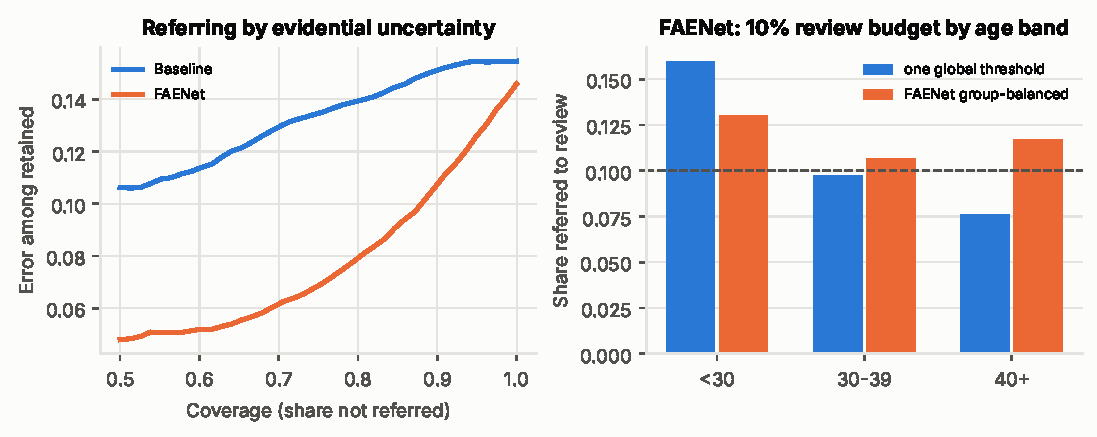
\includegraphics[width=0.78\textwidth]{uncertainty_review_final}
\caption{Left: error of the predictions that are not referred, as more employees are sent to review in order of evidential uncertainty. Right: share of each age band referred under one global threshold and under FAENet's group-balanced thresholds.}\label{fig:review}\end{figure*}

\subsection{Predictive Performance}
FAENet improves ROC-AUC from 0.814 to 0.827 (CI of the gain 0.004 to 0.024), PR-AUC from 0.575 to 0.604 (0.006 to 0.055) and precision from 0.520 to 0.549, while keeping recall at the same level (Table~\ref{tab:main}). The engineered tenure and satisfaction features, the milder class weights and the five-member ensemble all contribute. Calibration also improves: after Platt scaling the ECE is 0.020 and the Brier score falls from 0.101 to 0.095, so predicted risks can be read directly as attrition likelihoods. FAENet also clearly exceeds the 0.773 ROC-AUC reported for XGBoost on IBM by Jia \cite{jia2026}.

\subsection{Fairness Across Age Groups}
\begin{figure}[t]\centering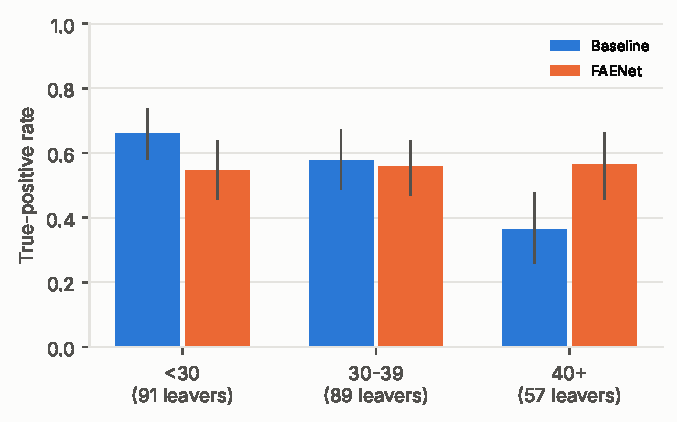
\includegraphics[width=0.92\columnwidth]{age_tpr_final}
\caption{True-positive rate by age band for the baseline and FAENet with age-aware thresholds (95\% CI).}\label{fig:age}\end{figure}
The baseline detects only 36.5\% of leavers aged 40+, against about 60\% in the younger groups. FAENet's age-aware thresholds raise detection in the 40+ group to 56.5\% (gain 0.200, CI 0.137 to 0.263), lift the worst age-band TPR from 0.365 to 0.519, and reduce the age-band TPR gap from 0.297 to 0.077 (Fig.~\ref{fig:age}). Leavers are therefore detected at closely similar rates in all three age groups, and FAENet predicts attrition well in every age band. Used during training, the equal-opportunity penalty ($\lambda_f=30$) narrows the gap further at the standard threshold, by 0.096, with ROC-AUC unchanged at 0.824. The gender TPR gap is small (0.062).

\subsection{Uncertainty and Human Review}
\begin{figure}[!t]\centering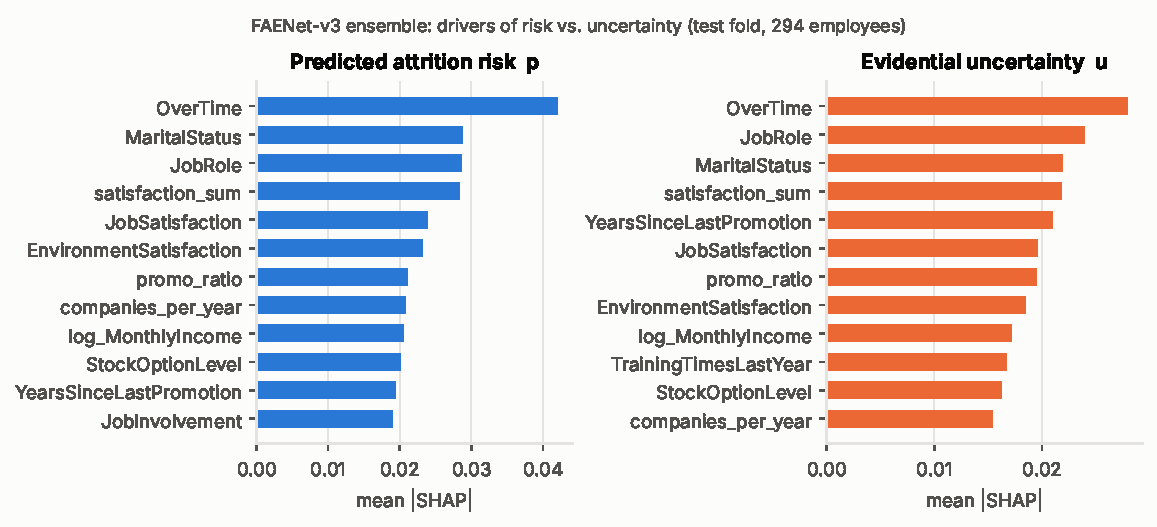
\includegraphics[width=\columnwidth]{shap_global}
\caption{Mean absolute SHAP values for FAENet's predicted risk and uncertainty.}\label{fig:shap}\end{figure}

FAENet's evidential uncertainty identifies misclassified employees with an AUROC of 0.790, against 0.612 for the baseline (gain 0.178, CI 0.144 to 0.205), and it also outperforms the margin to the decision threshold (0.712). As a result, referring the 10\% most uncertain employees lowers the error among the remaining predictions from 0.149 to 0.105, and the advantage holds at every review budget (Fig.~\ref{fig:review}, left). With a single global threshold, review would concentrate on employees under 30 (16\% referred against 8\% of those aged 40+); FAENet's group-balanced thresholds reduce this review-rate gap from 0.084 to 0.038 (Fig.~\ref{fig:review}, right), so human attention is shared fairly across age groups. When an entire department is excluded from training, FAENet's uncertainty rises for its employees (AUROC 0.584 for separating them from familiar employees), signalling unfamiliar cases.

\subsection{Explainability}

SHAP identifies overtime, marital status, job role, the engineered satisfaction sum, job satisfaction, environment satisfaction and promotion recency as the main drivers of predicted risk (Fig.~\ref{fig:shap}), consistent with prior findings \cite{talebi2025,alali2026}. Uncertainty is driven by a similar set of features, so the reasons behind each referral can be shown to the reviewer.

\FloatBarrier
\section{Conclusion and Future Work}
FAENet meets all five objectives. Compared with a single evidential network, it raises ROC-AUC to 0.827 and PR-AUC to 0.604, provides calibrated probabilities (ECE 0.020), raises detection of leavers aged 40+ from 0.365 to 0.565 while cutting the age-band gap from 0.297 to 0.077, identifies its own likely mistakes through evidential uncertainty (AUROC 0.790 against 0.612), and refers uncertain cases to human review in a balanced way across age groups, with SHAP explanations for every decision.

Future work will extend the evaluation to larger HR datasets with more leavers in each age group, since the current dataset contains only 57 leavers aged 40+, which limits how precisely group-level behaviour can be learned. Further directions are nested model selection, intersectional fairness (for example gender and age combined), richer behavioural and temporal features, and an interactive dashboard that presents risk, uncertainty, review flags and explanations to HR teams.

\section*{Declaration and Data Availability}
The authors declare no conflict of interest. The IBM HR Analytics dataset is publicly available at \url{https://www.kaggle.com/datasets/pavansubhasht/ibm-hr-analytics-attrition-dataset}. The code, configurations and experiment outputs are available at \url{https://github.com/akashagarwal07/FAENet}.

\FloatBarrier
\bibliographystyle{IEEEtran}
\bibliography{refs}
\end{document}
